\subsubsection{Dowód poprawności}
Twierdzenie 1.\\
	Każde drzewo można przejść wracajac do korzenia przeskakując maksymalnie dwa wierzchołki, tak aby każdy wierzchołek oprócz korzenia odwiedzić dokładnie raz.\\\\
Dowód:\\
	Dowód będzie polegał na zasadzie indukcji matematycznej.\\ Najpierw udowodnimy że dla podstawowych drzew 1,2,3 wierzchołkowych twierdzenie zachodzi.\\
	Następnie udowodnimy, że można takie grafy przejść na dwa sposoby:
	\begin{enumerate}[a.]
	\item Zaczynając od korzenia, można przejść przez wszystkie wierzchołki odwiedzając je dokładnie raz i kończąc na dziecku korzenia (oczywiście z dziecka korzenia zawsze można przejść do korzenia jako ostatni ruch zamykając cykl)
	\item Zaczynając od dziecka korzenia, można przejść przez wszystkie wierzchołki odwiedzając je dokładnie raz i kończąc na korzeniu
	\end{enumerate}
	Z tym, że jeśli graf jest jednowierzchołkowy, nie trzeba go oczywiście dalej przechodzić, jeśli już w niego weszliśmy. Natomiast grafu 0 wierzchołkowego nie trzeba przechodzić wogóle, więc napewno można go przejść na te dwa sposoby.\\\\

	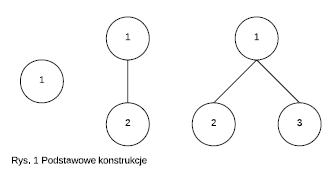
\includegraphics{rys1}\\\\
	
	Łatwo zauważyć, że dla tych podstawowych konstrukcji udowodnienie założeń jest banalne. Np. dla grafu z 2 wierzchołkami można przejść z 1 do 2 i z 2 do 1 albo odwrotnie.\\\\

	Następnie zakładamy, że umiemy przejść na te dwa sposoby drzewa A i B. Udowodnimy, że można przejść na te dwa sposoby większe drzewo C powstałe poprzez połączenie drzew A i B z nowym wierzchołkiem (jako korzeń). Ten sposób konstrukcji pozwala stworzyć dowolne drzewo. Jeśli udowodnimy, że z możliwości przejścia w te sposoby drzew A i B wynika, że mozna przejść drzewo C, co znaczy, że można przejść na te sposoby każde drzewo. \\\\

	Mamy dwa przypadki:
	\begin{enumerate}[1]
	\item Z korzenia przechodzimy do dziecka korzenia grafu A i przechodzimy go sposobem a), kończąc na korzeniu drzewa A. Następnie przechodzimy do dziecka korzenia drzewa B i przechodzimy go sposobem a), kończąc w korzeniu grafu B. W ten sposób skończyliśmy w dziecku powstałego drzewa C. W ten sposób udało się przejść drzewo C w sposób b).\\\\
	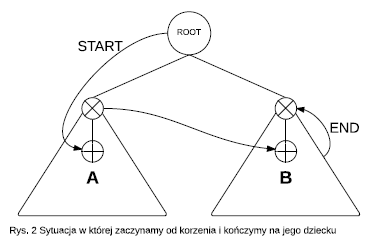
\includegraphics{rys2}\\\\

	\item Zaczynamy z dziecka grafu C, zatem z korzenia grafu np. A. Następnie przechodzimy graf A sposobem b) kończąc w dziecku korzenia drzewa A. Następnie przechodzimy przeskakując 2 wierzchołki (korzeń drzewa A i C) do korzenia drzewa B i znowu przechodzimy go sposobem b). Na koniec skaczemy przez korzeń drzewa B i kończymy w korzeniu drzewa C. W ten sposób przeszliśmy drzewo C na sposób a).\\\\
	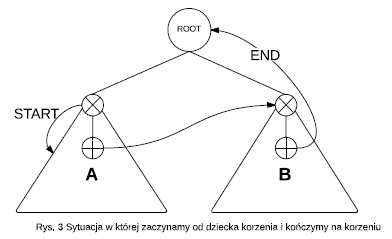
\includegraphics{rys3}\\\\
	\end{enumerate}
	Z indukcji matematycznej wynika, że każde drzewo da się przejść na sposób a) i b). Natomiast z możliwości przejścia na oba sposoby każdego drzewa wynika, że twierdzenie jest prawdziwe.\\\\
